\documentclass[14pt,a4paper]{extarticle}
% =============================================================
% preamble_compact.tex — компактный вариант оформления отчётов
% Основа — preamble.tex (СТП БГУИР); здесь только уплотнение:
% разделы без принудительного перехода на новую страницу,
% меньшие вертикальные отступы, плотные списки и подписи.
% =============================================================
% =============================================================
% preamble.tex — Shared LaTeX preamble for genetic/evolutionary reports
% Conforming to BSUIR STP 01-2024
% =============================================================

% Encoding and language
\usepackage[utf8]{inputenc}
\usepackage[T2A]{fontenc}
\usepackage[russian]{babel}

% Times New Roman font
\usepackage{tempora}

% Page geometry: STP 2.1.1
\usepackage{geometry}
\geometry{left=30mm, right=15mm, top=20mm, bottom=20mm}

% Line spacing: STP 2.1.1
\usepackage{setspace}
\singlespacing

% Allow TeX a bit more flexibility to avoid overflow
\pretolerance=1000
\tolerance=2000
\emergencystretch=3em

% Paragraph indent
\usepackage{indentfirst}
\setlength{\parindent}{1.25cm}

% Page numbers
\usepackage{fancyhdr}
\pagestyle{fancy}
\fancyhf{}
\fancyfoot[R]{\thepage}
\renewcommand{\headrulewidth}{0pt}
\fancypagestyle{plain}{%
  \fancyhf{}%
  \fancyfoot[R]{\thepage}%
  \renewcommand{\headrulewidth}{0pt}%
}

% Math
\usepackage{amsmath,amssymb}

% Graphics
\usepackage{graphicx}
\usepackage{float}
\usepackage{xcolor}

% Tables
\usepackage{booktabs}
\usepackage{tabularx}
\usepackage{multirow}
\usepackage{longtable}

% Captions
\usepackage{caption}
\captionsetup[figure]{
  labelsep=endash,
  justification=centering,
  font={normalsize},
  name=Рисунок
}
\captionsetup[table]{
  labelsep=endash,
  justification=raggedright,
  singlelinecheck=false,
  font={normalsize},
  name=Таблица
}

% Section formatting
\usepackage{titlesec}
\titleformat{\section}
  {\newpage\normalfont\fontsize{14}{18}\selectfont\bfseries}
  {\thesection}{0.5em}{\MakeUppercase}
\titlespacing*{\section}{1.25cm}{0pt}{14pt}

\titleformat{\subsection}
  {\normalfont\fontsize{14}{18}\selectfont\bfseries}
  {\thesubsection}{0.5em}{}
\titlespacing*{\subsection}{1.25cm}{14pt}{14pt}

\titleformat{\subsubsection}
  {\normalfont\fontsize{14}{18}\selectfont\bfseries}
  {\thesubsubsection}{0.5em}{}
\titlespacing*{\subsubsection}{1.25cm}{14pt}{14pt}

% Unnumbered sections
\newcommand{\sectioncenter}[1]{%
  \newpage
  \phantomsection
  \addcontentsline{toc}{section}{#1}
  \begin{center}
    \textbf{\MakeUppercase{#1}}
  \end{center}
  \vspace{14pt}
}

% Table of contents formatting
\usepackage{tocloft}
\renewcommand{\cftsecfont}{\normalfont}
\renewcommand{\cftsecpagefont}{\normalfont}
\renewcommand{\cftsubsecfont}{\normalfont}
\renewcommand{\cftsubsecpagefont}{\normalfont}
\renewcommand{\cftsecleader}{\cftdotfill{\cftdotsep}}
\renewcommand{\cftdotsep}{1}
\renewcommand{\contentsname}{\hfill\textbf{СОДЕРЖАНИЕ}\hfill}
\renewcommand{\cftaftertoctitle}{\hfill}

% Lists
\usepackage{enumitem}
\setlist[itemize]{noitemsep, topsep=0pt, leftmargin=1.25cm, label=--}
\setlist[enumerate]{noitemsep, topsep=0pt, leftmargin=1.25cm}

% Code listings
\usepackage{listings}
\usepackage{fancyvrb}
\lstset{
  basicstyle=\ttfamily\small,
  frame=single,
  breaklines=true,
  showstringspaces=false,
  inputencoding=utf8,
  extendedchars=true,
  literate={а}{{\cyra}}1 {б}{{\cyrb}}1 {в}{{\cyrv}}1 {г}{{\cyrg}}1
           {д}{{\cyrd}}1 {е}{{\cyre}}1 {ж}{{\cyrzh}}1 {з}{{\cyrz}}1
           {и}{{\cyri}}1 {й}{{\cyrishrt}}1 {к}{{\cyrk}}1 {л}{{\cyrl}}1
           {м}{{\cyrm}}1 {н}{{\cyrn}}1 {о}{{\cyro}}1 {п}{{\cyrp}}1
           {р}{{\cyrr}}1 {с}{{\cyrs}}1 {т}{{\cyrt}}1 {у}{{\cyru}}1
           {ф}{{\cyrf}}1 {х}{{\cyrh}}1 {ц}{{\cyrc}}1 {ч}{{\cyrch}}1
           {ш}{{\cyrsh}}1 {щ}{{\cyrshch}}1 {ъ}{{\cyrhrdsn}}1
           {ы}{{\cyrery}}1 {ь}{{\cyrsftsn}}1 {э}{{\cyrerev}}1
           {ю}{{\cyryu}}1 {я}{{\cyrya}}1
}

% Hyperlinks
\usepackage{hyperref}
\hypersetup{
  colorlinks=true,
  linkcolor=black,
  urlcolor=blue,
  citecolor=black,
}

% Number figures and tables within sections
\numberwithin{figure}{section}
\numberwithin{table}{section}
\numberwithin{equation}{section}

% Standard title page macro
\newcommand{\makegeclabtitle}[2]{%
  \begin{titlepage}
  \thispagestyle{empty}
  \begin{center}

  МИНИСТЕРСТВО ОБРАЗОВАНИЯ РЕСПУБЛИКИ БЕЛАРУСЬ

  \vspace{0.5em}

  Учреждение образования

  \vspace{0.5em}

  \textbf{<<Белорусский государственный университет информатики и радиоэлектроники>>}

  \vspace{2em}

  Факультет компьютерных систем и сетей

  \vspace{0.5em}

  Кафедра программного обеспечения информационных технологий

  \end{center}

  \vspace{3em}

  \begin{center}
  \textbf{ОТЧЕТ}

  \vspace{0.5em}

  по лабораторной работе №#1

  \vspace{0.5em}

  по дисциплине

  \vspace{0.5em}

  <<Генетические и эволюционные вычисления>>

  \vspace{0.5em}

  <<#2>>
  \end{center}

  \vspace{5em}

  \begin{flushright}
  \begin{minipage}{0.5\textwidth}
  \textbf{Выполнил:}\\
  Лебедевич Артем Владимирович\\
  магистрант группы 556301

  \vspace{0.6em}

  \textbf{Преподаватель:}\\
  Нестеренков Сергей Николаевич\\
  кандидат технических наук\\
  доцент кафедры ПОИТ
  \end{minipage}
  \end{flushright}

  \vfill

  \begin{center}
  Минск, 2026~г.
  \end{center}

  \end{titlepage}
}


% Разделы идут подряд, без \newpage
\titleformat{\section}
  {\normalfont\fontsize{14}{17}\selectfont\bfseries}
  {\thesection}{0.5em}{\MakeUppercase}
\titlespacing*{\section}{1.25cm}{12pt}{6pt}
\titlespacing*{\subsection}{1.25cm}{8pt}{4pt}

% Плотнее плавающие объекты и подписи
\setlength{\textfloatsep}{8pt plus 2pt minus 2pt}
\setlength{\floatsep}{6pt plus 2pt minus 2pt}
\setlength{\intextsep}{6pt plus 2pt minus 2pt}
\captionsetup[figure]{skip=3pt, font={small}}
\captionsetup[table]{skip=2pt, font={small}}
\setlength{\abovedisplayskip}{4pt}
\setlength{\belowdisplayskip}{4pt}

% Таблицы компактнее
\renewcommand{\arraystretch}{1.05}
\setlength{\tabcolsep}{5pt}

% Номера рисунков и таблиц — сквозные (без привязки к разделам)
\counterwithout{figure}{section}
\counterwithout{table}{section}
\counterwithout{equation}{section}

\graphicspath{{figures/}}

\begin{document}

\makegeclabtitle{4}{Кластеризация с помощью нейронной сети Кохонена}

\section{Цель работы}

Изучить архитектуру самоорганизующихся карт признаков (SOM) Кохонена, алгоритмы конкурентного обучения без учителя и получить навыки кластеризации двумерных данных с визуальным анализом топологии сети.

\section{Краткие теоретические сведения}

\textbf{Архитектура.} Карта~--- слой нейронов в узлах решётки; нейрон $i$ имеет вектор весов $W_i$ и положение $r_i$ на решётке. Топология \texttt{gridtop}~--- прямоугольная решётка (4 соседа), \texttt{hextop}~--- гексагональная (нечётные ряды сдвинуты на $1/2$, 6 соседей на одинаковом расстоянии). Расстояние на решётке \texttt{linkdist}~--- число связей по кратчайшему пути.

\textbf{Обучение.} Для входа $p$ определяется победитель $c$: $\lVert W_c - p \rVert = \min_i \lVert W_i - p \rVert$. Веса победителя и его соседей сдвигаются к входу:
\begin{equation}
W_i(t+1) = W_i(t) + \eta(t)\,h_{ci}(t)\,\bigl(p - W_i(t)\bigr).
\end{equation}
Основное правило~--- гауссова окрестность $h_{ci} = \exp(-\lVert r_c - r_i\rVert^2 / 2\sigma^2(t))$; радиус $\sigma$ убывает с половины диаметра решётки до $0{,}3$, скорость $\eta$~--- с $0{,}5$ до $0{,}01$. Для сравнения реализовано правило \texttt{learnsom} MATLAB (\texttt{newsom}): победитель получает $h = 1$, соседи в радиусе \texttt{nd}~--- $0{,}5$; в фазе упорядочивания $\eta$ падает с $0{,}9$ до $0{,}02$, а \texttt{nd}~--- до \texttt{tune\_nd} (по умолчанию 1), в фазе подстройки \texttt{nd = tune\_nd}.

\textbf{Качество карты.} Квантизационная ошибка $QE = \frac1N\sum_k \lVert p_k - W_{c(p_k)}\rVert$; топографическая ошибка $TE$~--- доля точек, у которых первый и второй ближайшие нейроны не соседи на решётке; <<мёртвые>> нейроны не выигрывают ни разу; U-матрица~--- среднее расстояние весов нейрона до весов соседей (большие значения отмечают границы кластеров); ARI~--- совпадение с истинным разбиением (1~--- полное).

\section{Ход работы}

\textbf{Выборка.} Вариант~3: 4 кластера с центрами $(\pm 0{,}5;\ \pm 0{,}5)$. Программно сгенерировано 47, 31, 48 и 46 точек с разбросом (СКО) $0{,}112$, $0{,}106$, $0{,}147$ и $0{,}130$~--- случайные значения из диапазонов 30--50 и $0{,}10$--$0{,}15$; всего 172 точки на плоскости $[-1;\ 1]^2$.

\textbf{Реализация.} Класс \texttt{KohonenSOM} на NumPy (\texttt{lab\_04.ipynb}, аналог \texttt{newsom}/\texttt{train}/\texttt{sim}): топологии \texttt{hextop} и \texttt{gridtop}, произвольный размер сетки, случайная инициализация весов на $[-1;\ 1]^2$, снимки весов каждые 10 эпох. Интерактивное приложение \texttt{app/som\_trainer.html} (JavaScript, Plotly.js) реализует требования к интерфейсу: выбор топологии, размера сетки и числа эпох; точки выборки и веса нейронов со связями сетки на плоскости $[-1;\ 1]^2$; перерисовка каждые 10--20 эпох; ползунок <<Задержка (мс)>> и кнопки <<Старт>>, <<Пауза>>, <<Сброс>> (рисунок~\ref{fig:app}).

\textbf{Карта 2$\times$2.} Начальная конфигурация соответствует числу кластеров: 4 нейрона, \texttt{hextop}, 200 эпох (рисунок~\ref{fig:anim2}, таблица~\ref{tab:centroids}).

\begin{figure}[H]
\centering
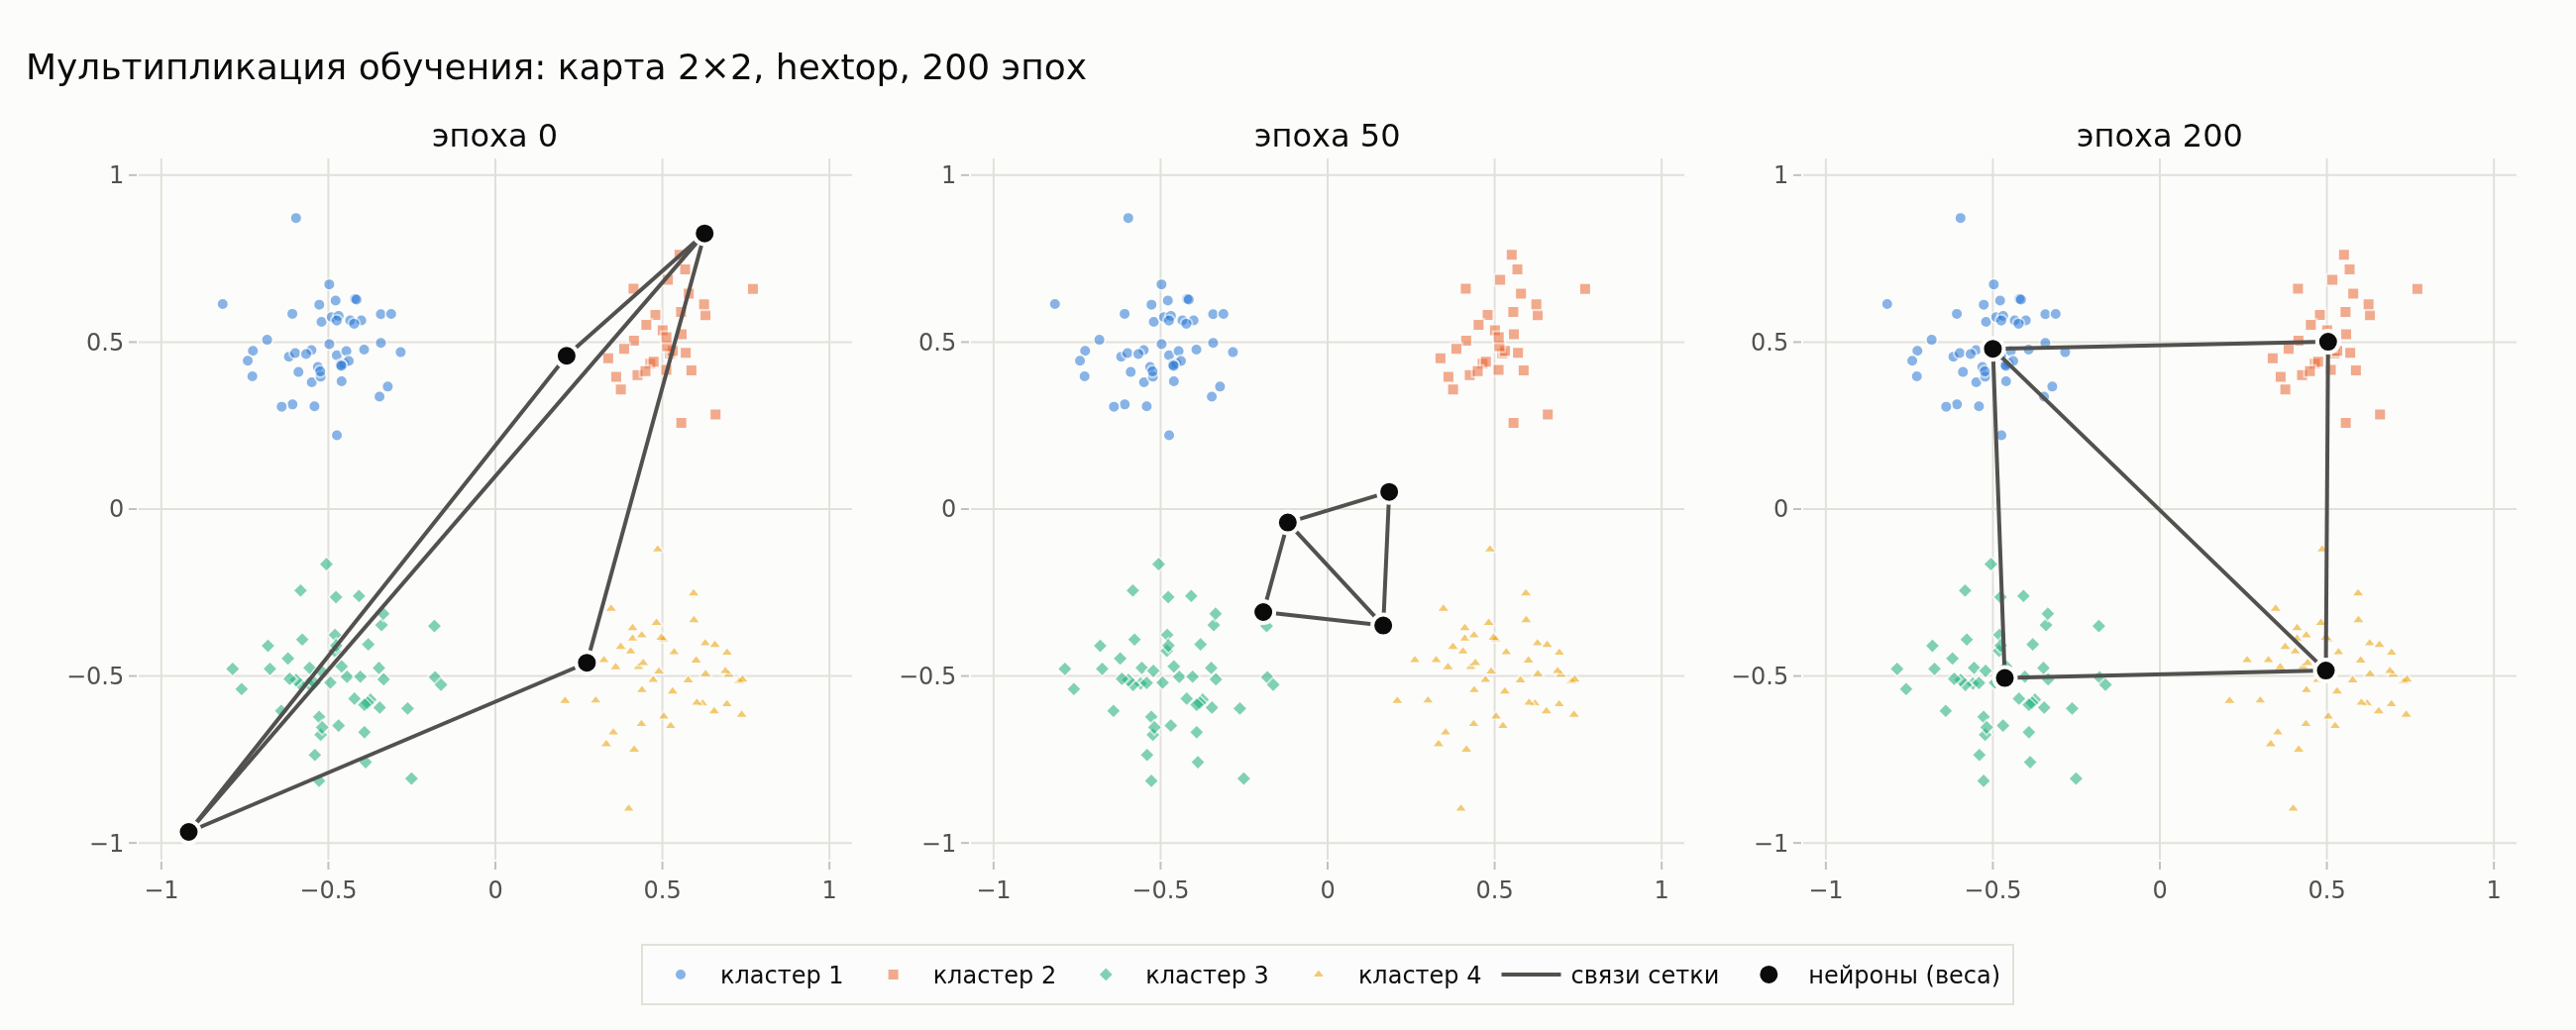
\includegraphics[width=\textwidth]{02_training_2x2_hextop.png}
\caption{Мультипликация обучения карты 2$\times$2 \texttt{hextop}: начальное, промежуточное и финальное положение нейронов}
\label{fig:anim2}
\end{figure}

\begin{table}[H]
\caption{Финальные центроиды карты 2$\times$2 hextop}
\label{tab:centroids}
\centering
\small
\begin{tabular}{cccccc}
\toprule
Нейрон & Кластер & Вес нейрона $(w_1; w_2)$ & Среднее кластера & Отклонение & Точек \\
\midrule
2 & 1 & (-0.500; +0.480) & (-0.506; +0.488) & 0.0102 & 47 \\
1 & 2 & (+0.504; +0.501) & (+0.511; +0.509) & 0.0109 & 31 \\
4 & 3 & (-0.464; -0.506) & (-0.469; -0.507) & 0.0051 & 48 \\
3 & 4 & (+0.497; -0.484) & (+0.506; -0.492) & 0.0122 & 46 \\
\bottomrule
\end{tabular}
\end{table}


Каждый нейрон занял центр своего облака: отклонение от среднего кластера~--- $0{,}005$--$0{,}012$. $QE = 0{,}157$ совпадает с k-means, ARI~$= 1$, $TE = 0$.

\textbf{Серия экспериментов.} Сетки 1$\times$4, 2$\times$2, 3$\times$3, 5$\times$5 в обеих топологиях, по 10 запусков (таблица~\ref{tab:series}, рисунок~\ref{fig:series}).

\begin{table}[H]
\caption{Серия экспериментов (правило gauss, 200 эпох, 10 запусков)}
\label{tab:series}
\centering
\small
\begin{tabular}{lccccc}
\toprule
Конфигурация & Нейронов & QE & TE & Мёртвых & ARI \\
\midrule
1$\times$4 gridtop & 4 & 0.1573 $\pm$ 0.0001 & 0.241 $\pm$ 0.036 & 0.0 & 1.000 \\
1$\times$4 hextop & 4 & 0.1573 $\pm$ 0.0001 & 0.241 $\pm$ 0.036 & 0.0 & 1.000 \\
2$\times$2 gridtop & 4 & 0.1573 $\pm$ 0.0000 & 0.000 $\pm$ 0.000 & 0.0 & 1.000 \\
2$\times$2 hextop & 4 & 0.1574 $\pm$ 0.0001 & 0.000 $\pm$ 0.000 & 0.0 & 1.000 \\
3$\times$3 gridtop & 9 & 0.1346 $\pm$ 0.0005 & 0.017 $\pm$ 0.008 & 1.0 & 1.000 \\
3$\times$3 hextop & 9 & 0.1344 $\pm$ 0.0031 & 0.000 $\pm$ 0.000 & 0.0 & 1.000 \\
5$\times$5 gridtop & 25 & 0.0765 $\pm$ 0.0010 & 0.108 $\pm$ 0.011 & 3.7 & 1.000 \\
5$\times$5 hextop & 25 & 0.0763 $\pm$ 0.0009 & 0.022 $\pm$ 0.014 & 2.9 & 1.000 \\
\bottomrule
\end{tabular}
\end{table}


\begin{figure}[H]
\centering
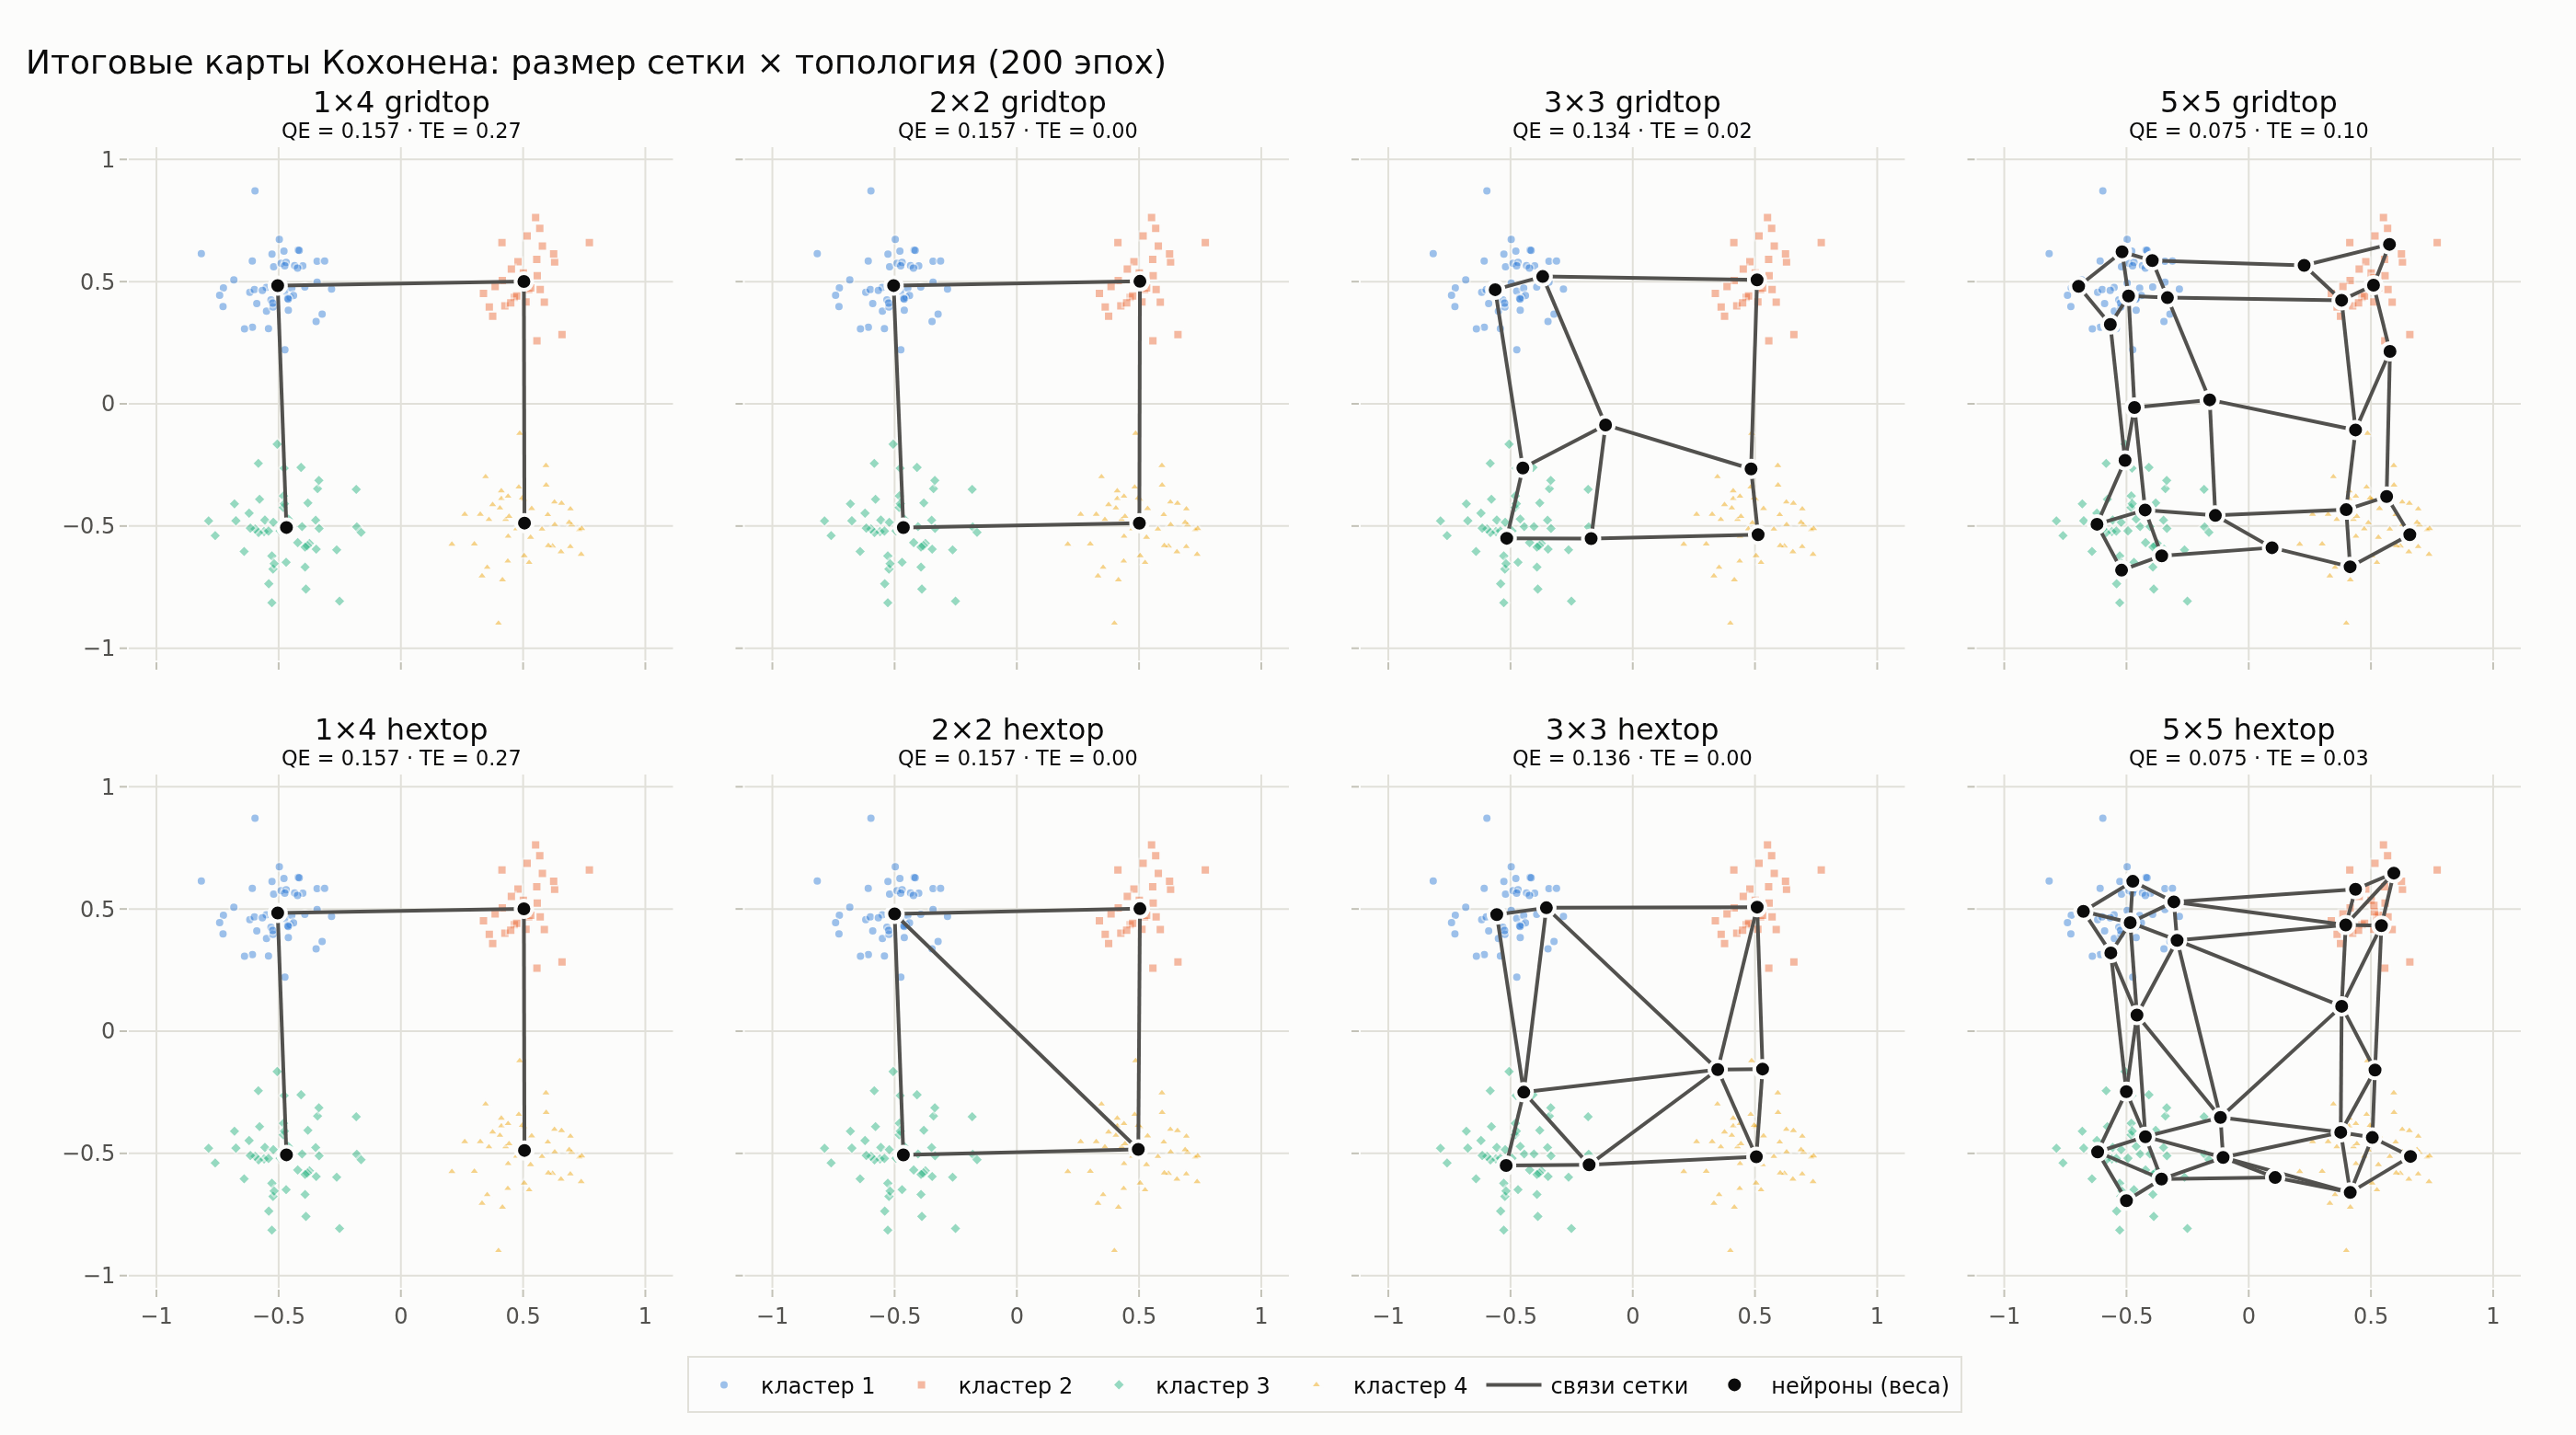
\includegraphics[width=\textwidth]{03_series_maps.png}
\caption{Итоговые карты: размер сетки $\times$ топология}
\label{fig:series}
\end{figure}

\textbf{Избыточная карта 5$\times$5.} Хаотичная сетка за 30--50 эпох упорядочивается в ровную решётку, затем растягивается к облакам и распределяется внутри них (рисунок~\ref{fig:anim5}). Число нейронов на облако пропорционально числу его точек (рисунок~\ref{fig:umatrix}, справа); 3--4 нейрона остаются между облаками без точек, и на U-матрице (рисунок~\ref{fig:umatrix}) они образуют границу четырёх кластеров.

\begin{figure}[H]
\centering
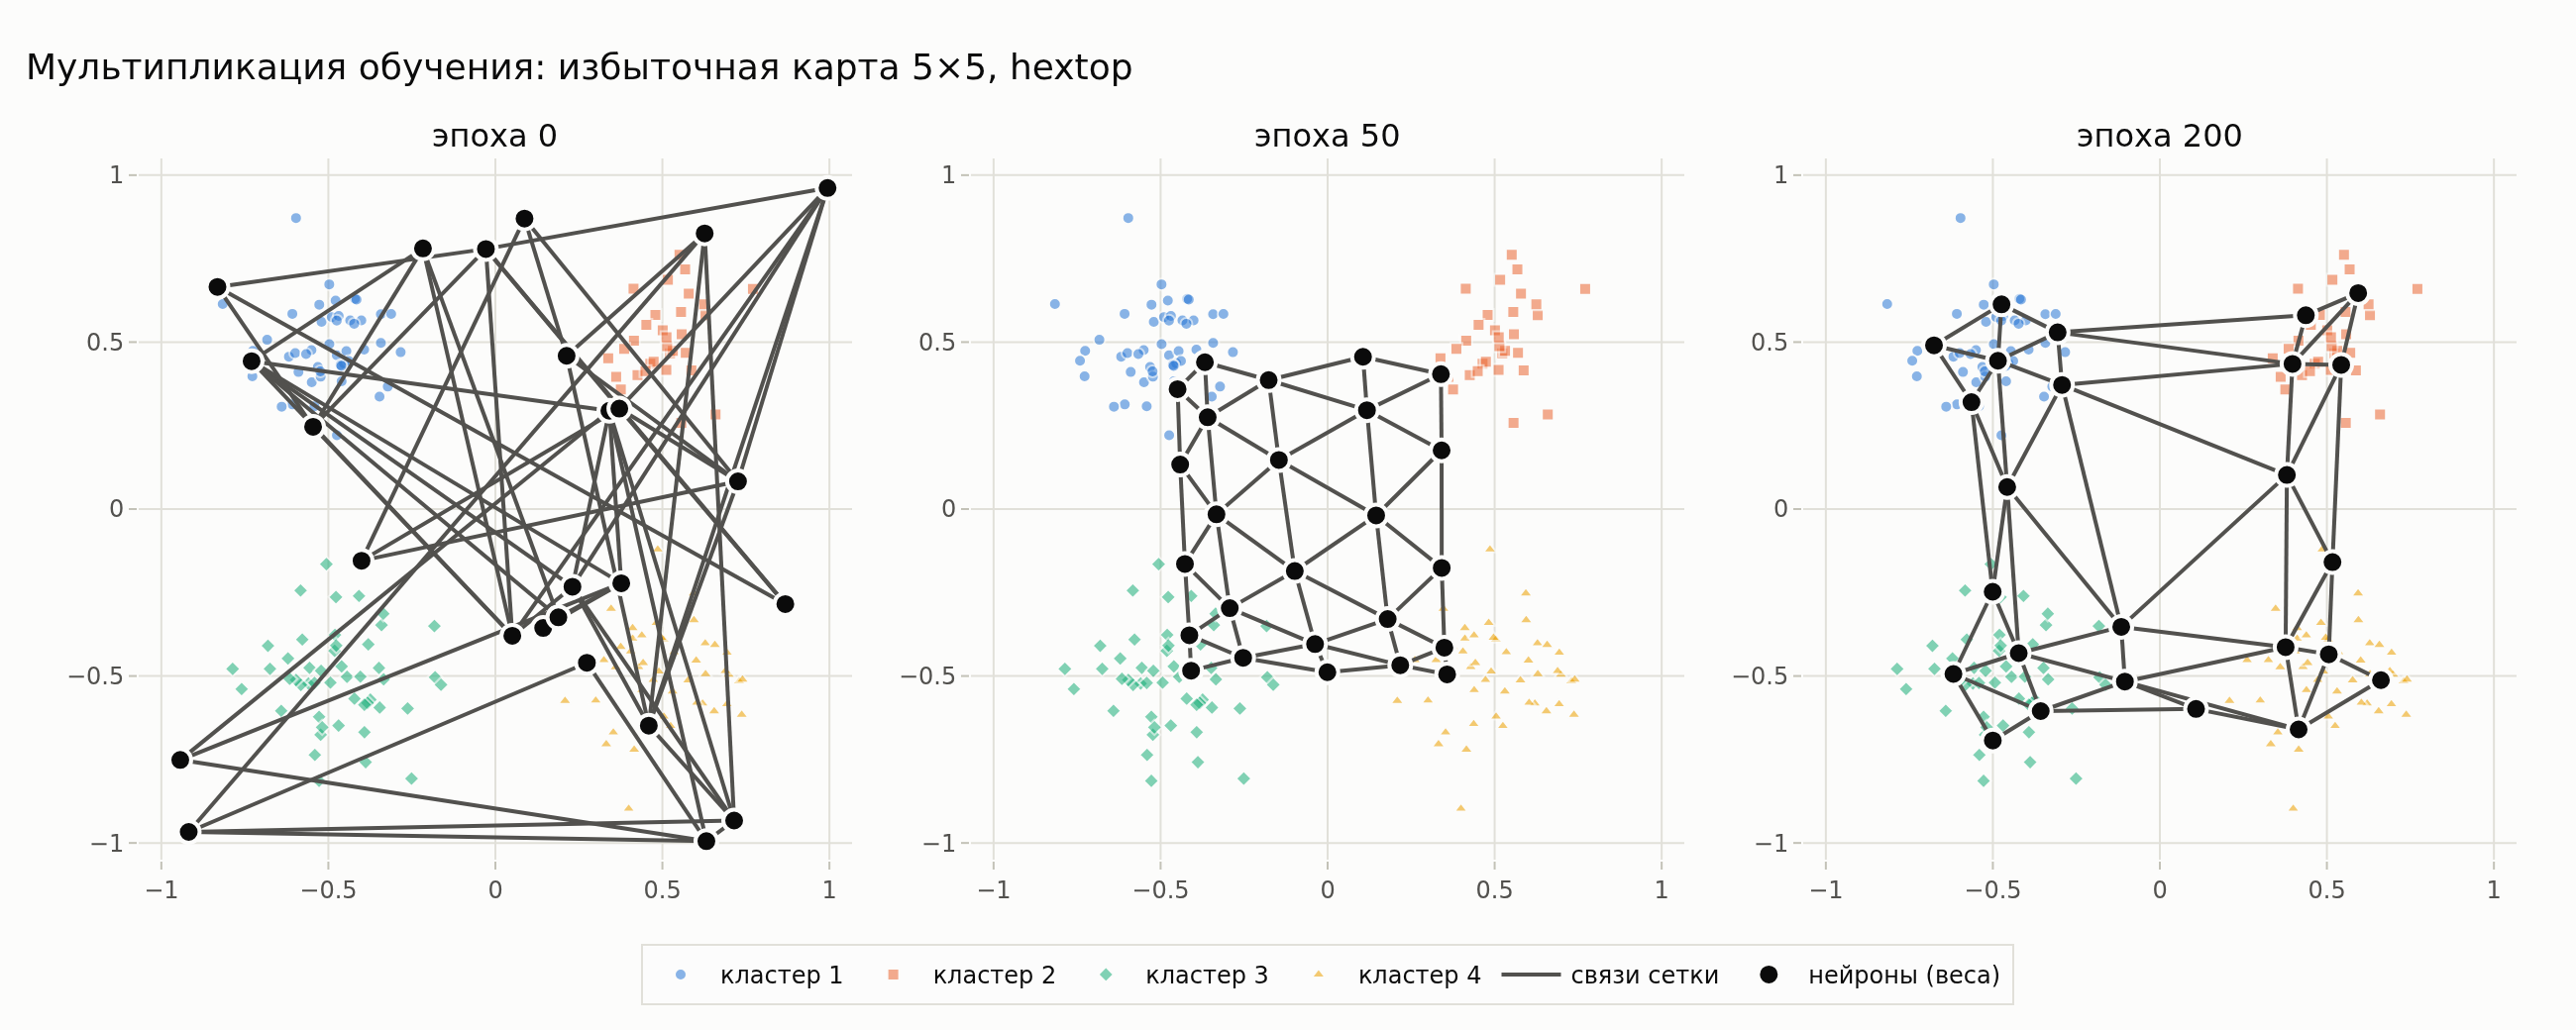
\includegraphics[width=\textwidth]{05_training_5x5_hextop.png}
\caption{Мультипликация обучения избыточной карты 5$\times$5 \texttt{hextop}}
\label{fig:anim5}
\end{figure}

\begin{figure}[H]
\centering
\begin{minipage}[c]{0.5\textwidth}\centering
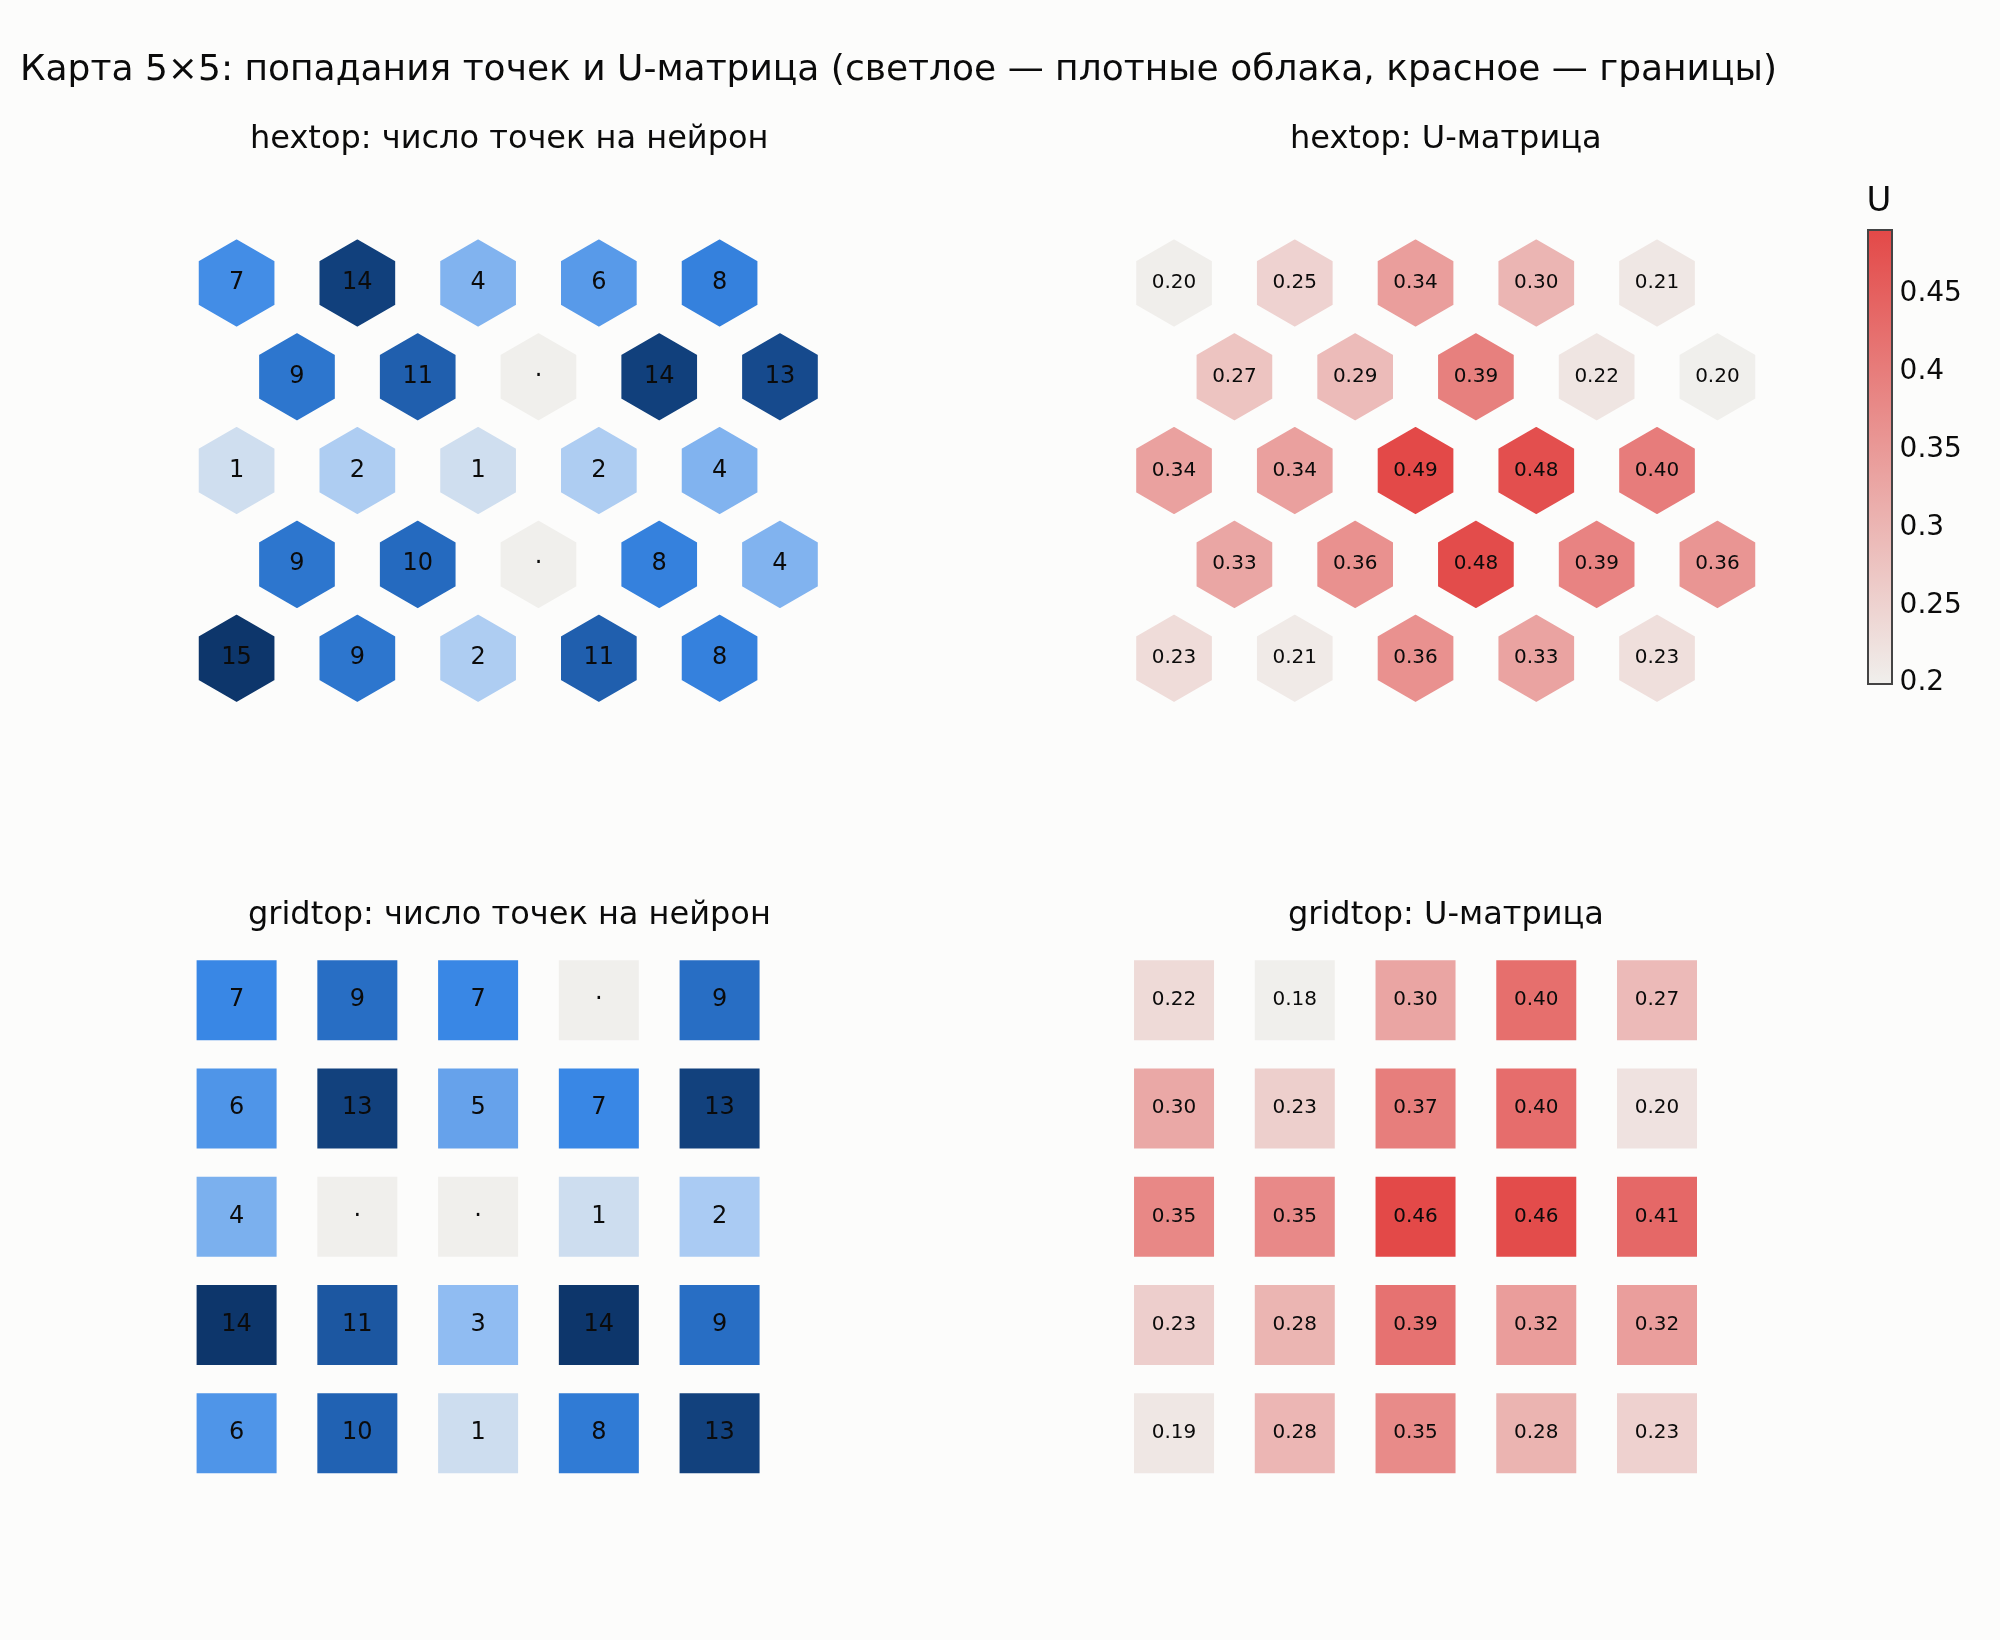
\includegraphics[width=\textwidth]{06_hits_umatrix.png}
\end{minipage}\hfill
\begin{minipage}[c]{0.47\textwidth}
\label{tab:share}\small\centering
\begin{tabular}{cccc}
\toprule
Кл. & Точек & grid & hex \\
\midrule
1 & 47 & 6.0 & 6.0 \\
2 & 31 & 3.3 & 3.5 \\
3 & 48 & 6.0 & 6.4 \\
4 & 46 & 6.0 & 6.2 \\
\bottomrule
\end{tabular}

\end{minipage}
\caption{Карта 5$\times$5: число точек на нейрон и U-матрица; справа~--- распределение нейронов по кластерам (среднее по 10 запускам)}
\label{fig:umatrix}
\end{figure}

\textbf{Правило обучения и число эпох.} В реплике \texttt{newsom} с \texttt{tune\_nd = 1} у карты 2$\times$2 все нейроны остаются соседями до конца обучения и тянут друг друга: центроиды стягиваются к центру плоскости, $QE = 0{,}38$--$0{,}46$ вместо $0{,}157$ (рисунок~\ref{fig:rules}). При \texttt{tune\_nd = 0} центры находятся точно, но у 5$\times$5 \texttt{gridtop} рвётся топология ($TE = 0{,}20$); гауссово правило даёт $QE = 0{,}076$ при $TE = 0{,}02$ (\texttt{hextop}). По числу эпох: уже через 20 эпох $QE$ отличается от итоговой на 1--8\,\%, после 100 эпох почти не меняется.

\begin{figure}[H]
\centering
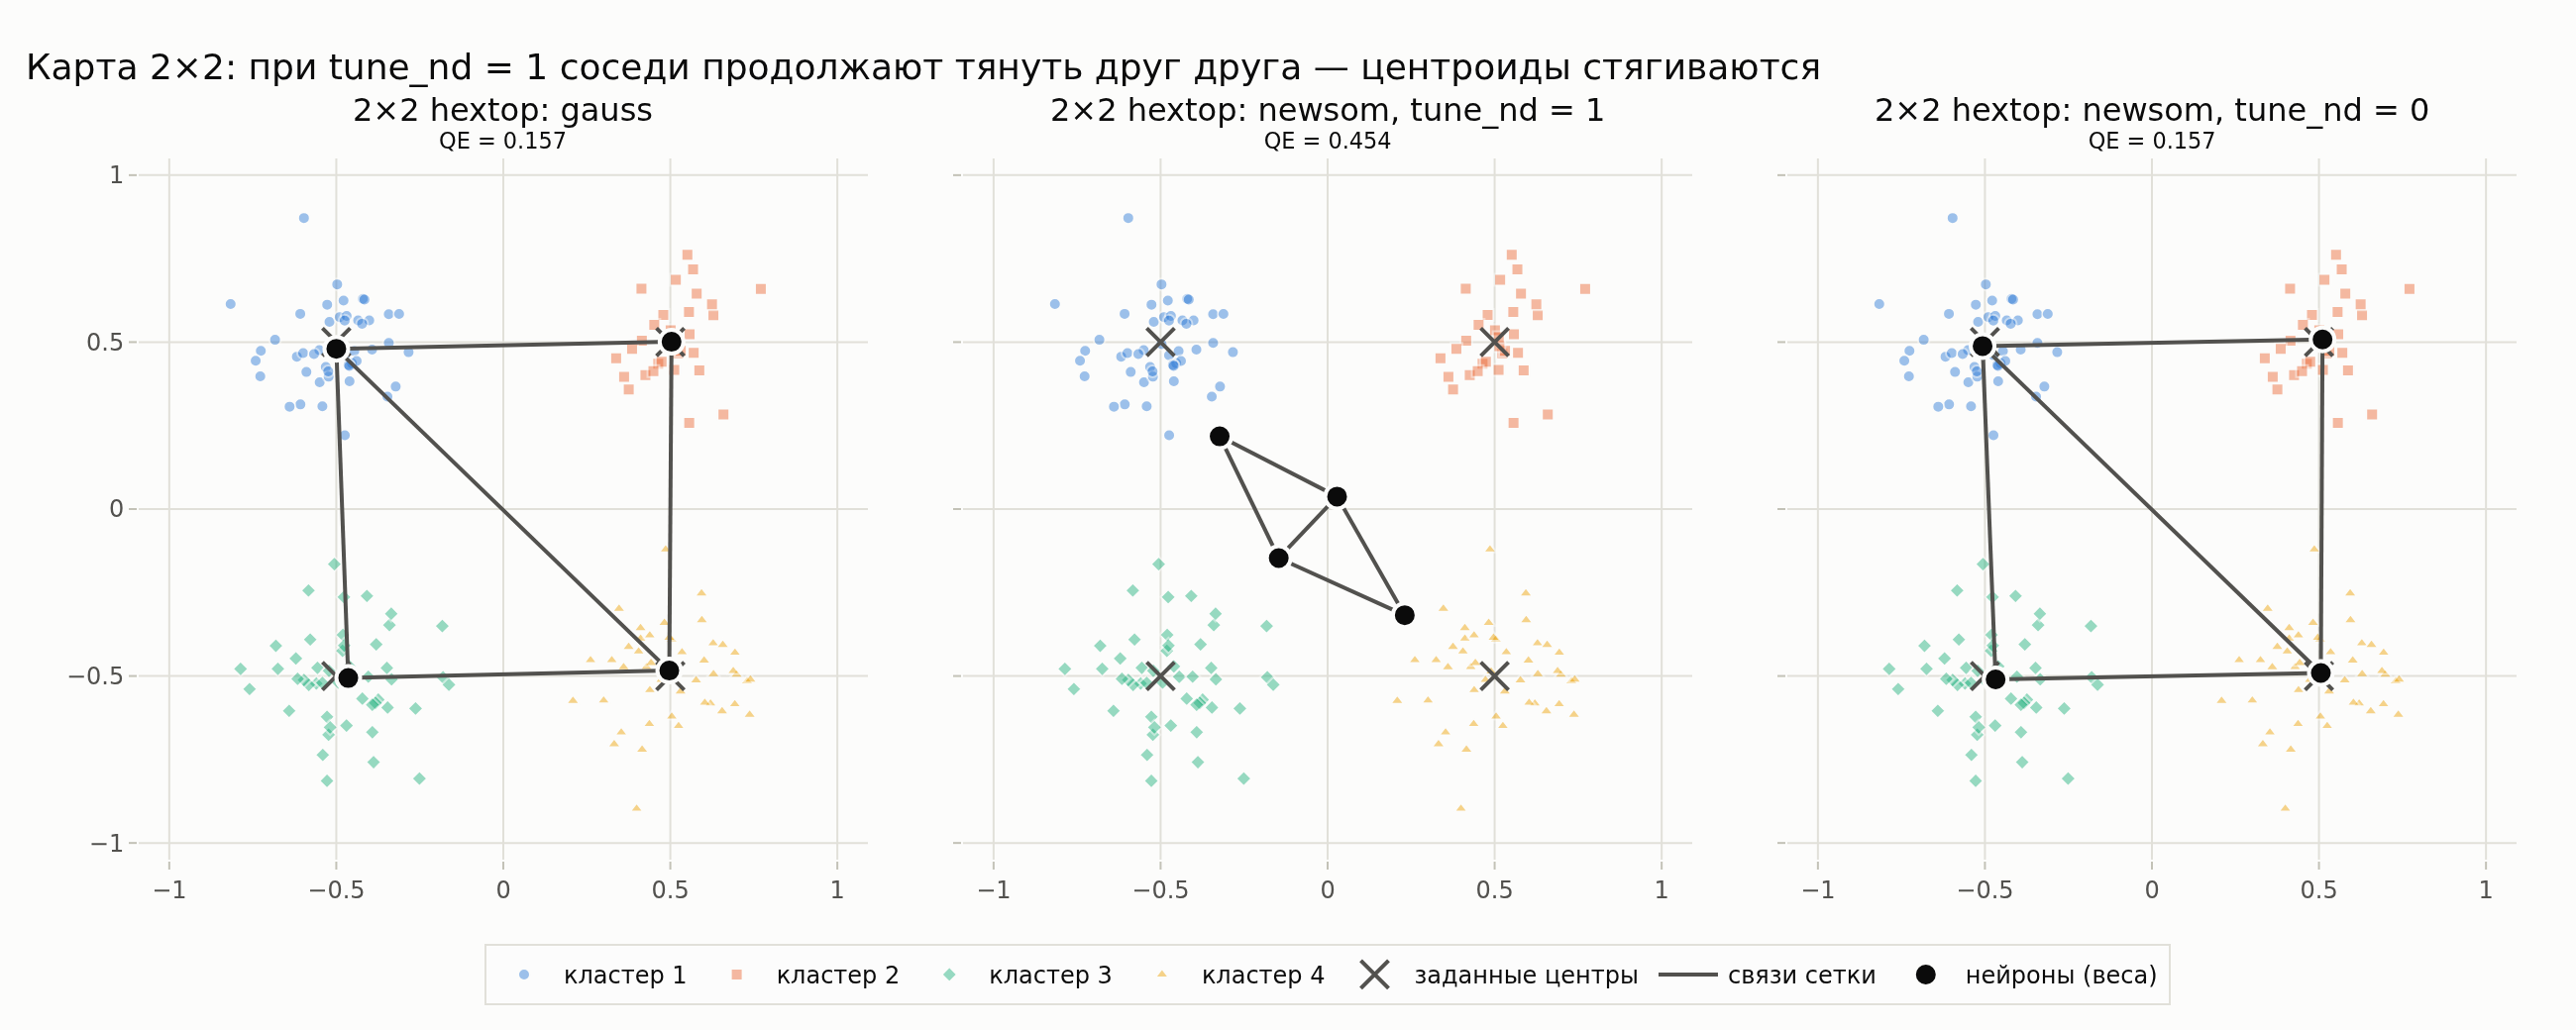
\includegraphics[width=\textwidth]{07_rules_2x2.png}
\caption{Карта 2$\times$2 при разных правилах обучения}
\label{fig:rules}
\end{figure}

\begin{figure}[H]
\centering
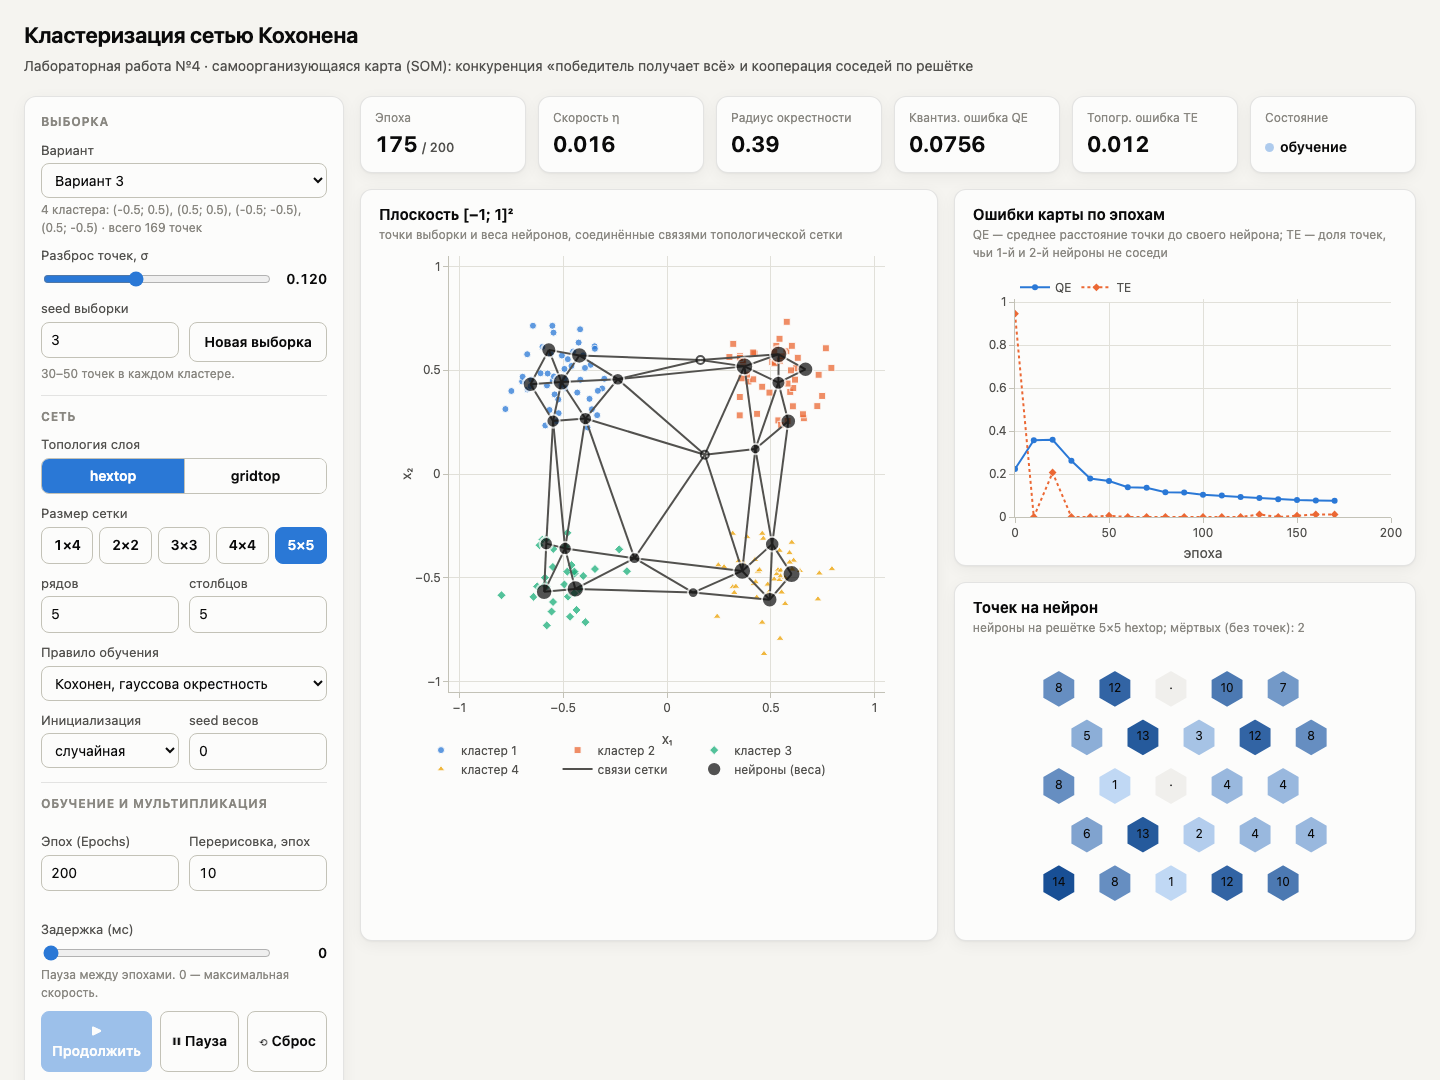
\includegraphics[width=0.72\textwidth]{00_app_screenshot.png}
\caption{Интерактивное приложение \texttt{app/som\_trainer.html}}
\label{fig:app}
\end{figure}

\section{Выводы}

\begin{enumerate}
\item Карта с числом нейронов, равным числу кластеров (2$\times$2), обучением без учителя находит центры кластеров с точностью k-means ($QE = 0{,}157$, ARI~$= 1$).
\item Избыточная карта 5$\times$5 растягивается по данным и воспроизводит их плотность; межкластерные нейроны и U-матрица выявляют границы кластеров.
\item Топология \texttt{hextop} сохраняет порядок нейронов лучше \texttt{gridtop}: $TE = 0{,}022$ против $0{,}108$ на 5$\times$5 при одинаковой $QE$.
\item Окрестность, не сужающаяся к концу обучения (\texttt{tune\_nd = 1}), стягивает маленькую карту к центру; гауссова окрестность обеспечивает и точность, и сохранение топологии.
\end{enumerate}

\section{Ответы на контрольные вопросы}

\textbf{1. Каков биологический аналог структурной организации самоорганизующихся карт Кохонена?} Топографические карты коры головного мозга (соматотопические, ретинотопические, тонотопические): соседние участки коры реагируют на близкие стимулы. Такая организация возникает за счёт латеральных связей: ближние нейроны возбуждают друг друга, дальние тормозят. В SOM это моделируют решётка нейронов, функция окрестности и конкуренция.

\textbf{2. Объясните математический принцип стратегии обучения <<Победитель получает всё>>.} Активируется один нейрон $c = \arg\min_i \lVert W_i - p\rVert$; только его веса сдвигаются к входу: $W_c \leftarrow W_c + \eta(p - W_c)$. Нейрон, побеждающий на группе точек, смещается к их среднему, т.е. минимизирует квантизационную ошибку (стохастический k-means). Недостаток~--- мёртвые нейроны; SOM устраняет его, обучая на ранних эпохах и соседей победителя.

\textbf{3. Как функция окрестности $h_{ci}$ и сетка (hextop/gridtop) влияют на изменение весов соседей?} $h_{ci}$ задаёт долю шага соседа в зависимости от расстояния \emph{на решётке}. При большом радиусе движется вся карта~--- она упорядочивается; при малом обучение локально, и нейроны подстраиваются под облака. Сетка определяет соседей: у \texttt{hextop} их 6 на равном расстоянии, поэтому карта изгибается равномернее ($TE = 0{,}02$ против $0{,}11$ у \texttt{gridtop}). Если окрестность не сужается до нуля, соседи продолжают тянуть друг друга, и центроиды маленькой карты стягиваются.

\textbf{4. Что происходит с картой при избыточном количестве нейронов?} Карта растягивается по данным: нейроны распределяются внутри облаков пропорционально плотности (около 6 нейронов на облако из 46--48 точек и 3,4~--- на облако из 31 точки), облака дробятся на подкластеры, $QE$ падает с $0{,}157$ до $0{,}076$. Часть нейронов остаётся между облаками без точек: их удерживают связи решётки. Кластеры восстанавливаются объединением соседних нейронов по U-матрице.

\textbf{5. Почему сеть Кохонена обучается без учителя и откуда она извлекает информацию о структуре данных?} В алгоритме нет целевых выходов и ошибки <<выход~--- цель>>: веса меняются только по входам. Информацию сеть берёт из взаимного расположения точек (близость определяет победителя) и частоты векторов из разных областей (плотные области притягивают больше нейронов); функция окрестности превращает эту статистику в упорядоченную карту.

\end{document}
